\documentclass[12pt,a4paper]{article}

% --- Packages (same set and page setup as the Lab 1 report) ---
\usepackage[utf8]{inputenc}
\usepackage[T1]{fontenc}
\usepackage{lmodern}
\usepackage[english]{babel}
\usepackage[top=2.5cm,bottom=2.5cm,left=2.5cm,right=2.5cm]{geometry}
\usepackage{graphicx}
\usepackage{booktabs}
\usepackage{tabularx}
\usepackage{array}
\usepackage{float}
\usepackage{caption}
\usepackage{enumitem}
\usepackage{listings}
\usepackage{xcolor}
\usepackage{fancyhdr}
\usepackage[many]{tcolorbox}
\usepackage{microtype}
\usepackage{amsmath,amssymb}
\usepackage{tikz}
\usetikzlibrary{positioning,arrows.meta}
\usepackage{hyperref}

% --- Colours ---
\definecolor{primary}{RGB}{18,52,86}
\definecolor{secondary}{RGB}{41,128,185}
\definecolor{accent}{RGB}{231,76,60}
\definecolor{codebg}{RGB}{247,249,250}
\definecolor{codeframe}{RGB}{209,213,219}
\definecolor{codegray}{RGB}{108,117,125}
\definecolor{termgreen}{RGB}{80,250,123}
\definecolor{termred}{RGB}{255,85,85}
\definecolor{termyellow}{RGB}{241,250,140}

\hypersetup{colorlinks=true,linkcolor=primary,citecolor=secondary,urlcolor=secondary}

% --- Listings ---
\lstdefinestyle{code}{
    backgroundcolor=\color{codebg},
    basicstyle=\small\ttfamily,
    keywordstyle=\color{secondary}\bfseries,
    stringstyle=\itshape,
    commentstyle=\itshape\color{codegray},
    numbers=left,
    numberstyle=\tiny\color{codegray},
    numbersep=8pt,
    frame=single,
    rulecolor=\color{codeframe},
    breaklines=true,
    breakatwhitespace=true,
    showstringspaces=false,
    tabsize=4,
    captionpos=b
}
\lstdefinestyle{plain}{
    backgroundcolor=\color{codebg},
    basicstyle=\small\ttfamily,
    frame=single,
    rulecolor=\color{codeframe},
    breaklines=true,
    showstringspaces=false,
    captionpos=b
}
\lstdefinestyle{term}{
    backgroundcolor=\color{codebg},
    basicstyle=\small\ttfamily,
    frame=single,
    rulecolor=\color{codeframe},
    breaklines=true,
    showstringspaces=false,
    captionpos=b
}

% --- Terminal window (as in the Lab 1 report) ---
\tcbuselibrary{listings,skins}
\newtcblisting{terminalwindow}[1][]{%
    enhanced,
    colback=black,
    colframe=black,
    arc=2.5mm,
    boxrule=1pt,
    title={\textcolor{termred}{$\bullet$}\;\textcolor{termyellow}{$\bullet$}\;\textcolor{termgreen}{$\bullet$}\quad \textsf{\bfseries Console Terminal Session}},
    fonttitle=\small\sffamily\bfseries,
    coltitle=white,
    attach boxed title to top left={yshift=-2mm, xshift=4mm},
    boxed title style={colback=gray!15!black, arc=1.5mm, boxrule=0.5pt},
    listing only,
    listing options={
        backgroundcolor=\color{black},
        basicstyle=\small\ttfamily\color{white},
        frame=none,
        numbers=none,
        breaklines=true,
        tabsize=4,
        showspaces=false,
        showstringspaces=false,
        keepspaces=true
    },
    #1
}

% --- Header and footer: page number only, no header rule ---
\lstset{style=plain}

\pagestyle{fancy}
\fancyhf{}
\setlength{\headheight}{15pt}
\addtolength{\topmargin}{-3pt}
\fancyfoot[C]{\thepage}
\renewcommand{\headrulewidth}{0pt}
\renewcommand{\footrulewidth}{0pt}

\newcommand{\studentgroup}{FAF-241}

\begin{document}

% ======================================================================
% TITLE PAGE
% ======================================================================
\begin{titlepage}
  \centering
  {\large \textbf{TECHNICAL UNIVERSITY OF MOLDOVA}}\\[0.2cm]
  {\large Faculty of Computers, Informatics and Microelectronics}\\[0.2cm]
  {\large Department of Software Engineering and Automatics}\\[0.8cm]

  
\includegraphics[width=3.5cm]{figures/utm_logo.png}\\[1.2cm]

  {\Large \textbf{LABORATORY WORK NO. 4}}\\[0.4cm]
  {\LARGE \textbf{A Message Broker:\\ HTTP Streaming and gRPC}}\\[0.5cm]
  {\large Course: Network Programming}\\[2.5cm]

  \begin{minipage}{0.52\textwidth}
    \flushleft
    \textbf{Authors:}\\
    Dinu \textsc{Plesu}\\
    Igor \textsc{Boltunov}\\
    Student group: \studentgroup
  \end{minipage}
  \hfill
  \begin{minipage}{0.40\textwidth}
    \flushright
    \textbf{Verified by:}\\
    Lecturer / Supervisor\\
    Fistic Cristofor
  \end{minipage}

  \vfill
  {\large Chi\c{s}in\u{a}u --- 2026}
\end{titlepage}

\tableofcontents
\newpage

% ======================================================================
\section{Introduction}
% ======================================================================
In publish--subscribe, producers send events to a topic without knowing who
reads them, and consumers subscribe without knowing who writes. A broker in the
middle decouples the two sides in space, time and synchronisation.
That decoupling lets either side stop, restart or scale on its own, which is why
brokers sit at the centre of many event-driven systems.

The laboratory asks for such a broker, with two restrictions: no existing broker
product or messaging library may be used, and the broker must run on the
standard HTTP server of the language in Part~1 and on gRPC in Part~2. The
learning goal is therefore the mechanisms behind a correct broker: per-topic
ordering, unique identifiers, background fan-out, persistence across restarts,
and publisher authentication.

The work pursues four objectives:
\begin{enumerate}[itemsep=1pt]
  \item accept messages on named topics, assign per-topic identifiers and
        timestamps, and answer without waiting for subscribers;
  \item deliver each message in the background to every subscriber of its topic,
        while publishers and subscribers start and stop independently;
  \item keep messages and identifier continuity across a broker restart;
  \item restrict publishing with bearer tokens and return the correct HTTP and
        gRPC error codes.
\end{enumerate}

% ======================================================================
\section{Background}
% ======================================================================
\textbf{Publish--subscribe.} The pattern replaces direct coupling with an
intermediary that routes events by topic. Production brokers add
partitioning, replication and consumer groups. The laboratory
excludes these features on purpose. The work covers the core semantics only:
topics, ordering, fan-out, persistence and tokens.

\textbf{HTTP streaming.} An HTTP response body can be produced incrementally
. In Part~1 a subscriber sends a \texttt{GET} and the
broker keeps the response open, writing one JSON object per line. A publish
returns \texttt{202 Accepted} rather than \texttt{200 OK}, because the message is
queued and not yet delivered.

\textbf{gRPC.} gRPC uses Protocol Buffers as its interface language and HTTP/2
as its transport. A server-streaming call keeps one
HTTP/2 stream open and sends typed messages, which is the equivalent of the open
HTTP response. The generated stubs replace hand-written paths, status-code
conventions and JSON field names.

\textbf{Durability and tokens.} A single-node broker is durable if it writes its
state before acknowledging a publish, replaces the old file in one step, and does
not acknowledge a publish that it could not write. Bearer tokens travel in the
\texttt{Authorization} header or in the \texttt{authorization} metadata.

% ======================================================================
\section{Design}
% ======================================================================
Figure~\ref{fig:topology} shows the topology. Publishers and subscribers know
only the broker. The broker owns the topics, the delivery queue, persistence and
token checks. Both parts share this design, and only the transport differs.

\begin{figure}[H]
\centering
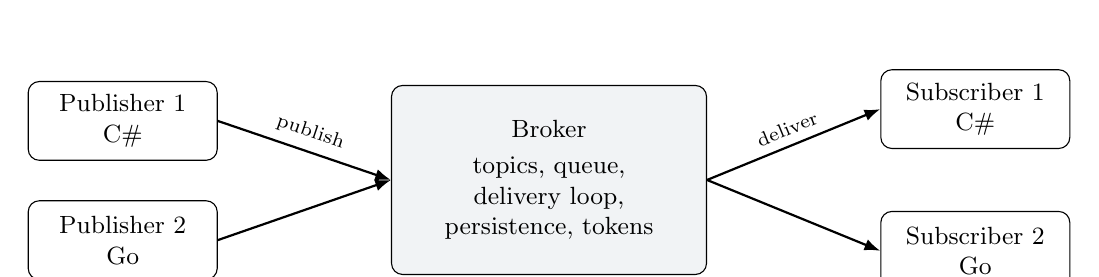
\begin{tikzpicture}[
  node distance=1.8cm,
  box/.style={draw, rounded corners, minimum width=2.4cm, minimum height=1.0cm,
              align=center, fill=white, font=\small},
  broker/.style={draw, rounded corners, minimum width=4.0cm, minimum height=2.4cm,
                 align=center, fill=primary!6, font=\small},
  arrow/.style={-{Latex[length=2mm]}, thick}
]
\node[box] (p1) {Publisher 1\\C\#};
\node[box, below=0.5cm of p1] (p2) {Publisher 2\\Go};
\node[broker, right=2.2cm of p1, yshift=-0.75cm] (b)
  {Broker\\[2pt]topics, queue,\\delivery loop,\\persistence, tokens};
\node[box, right=2.2cm of b, yshift=0.9cm] (s1) {Subscriber 1\\C\#};
\node[box, right=2.2cm of b, yshift=-0.9cm] (s2) {Subscriber 2\\Go};
\draw[arrow] (p1.east) -- node[above, font=\scriptsize, sloped]{publish} (b.west);
\draw[arrow] (p2.east) -- (b.west);
\draw[arrow] (b.east) -- node[above, font=\scriptsize, sloped]{deliver} (s1.west);
\draw[arrow] (b.east) -- (s2.west);
\end{tikzpicture}
\caption{Publishers and subscribers know only the broker, which owns the queue,
delivery loop, persistence and token checks.}
\label{fig:topology}
\end{figure}

\subsection{Identifiers and ordering}
Each topic has its own sequence. If $id(m_k)$ is the identifier of the $k$-th
message on a topic, then $id(m_1)=1$ and $id(m_{k+1})=id(m_k)+1$. The broker
assigns the identifier, stamps the time, appends the message, writes the topic's
file and queues the delivery while it holds a publish lock for that topic. Two
publishers on the same topic therefore never receive the same identifier, the
sequence has no gaps, and every subscriber receives the messages of a topic in
identifier order.

\subsection{Delivery}
A publish is answered once its message is saved and queued. One delivery loop
takes the queued messages in order and writes each one to the subscribers of its
topic. The loop copies the subscriber list under the topic lock and writes outside
it. A subscriber that cannot take a write is removed and logged; in the Go brokers
so is one whose 64-message buffer is full. The others still receive the message.
The Go brokers hold up to 1024 messages between the publishers and the delivery
loop, and a publish waits only when that queue is full. The C\# brokers queue
without a limit.

\subsection{Persistence}
After each accepted message the broker writes the topic to
\path{broker-data/<topic>/messages.json}. It writes a temporary file and then
renames it over the old file, so a crash during the write leaves the previous
file intact; the Go brokers also flush the file to disk before the rename. The
write happens while the publish lock is held, so the file always holds the latest
state. If the write fails, the message is taken out of memory again and the
publish is answered with 500 (HTTP) or \texttt{Internal} (gRPC), so no message is
acknowledged that is not on disk. On startup the broker loads every topic and sets
the next identifier to $\max(id)+1$.

\subsection{Tokens}
The broker reads \texttt{tokens.txt}, one entry per line:
\texttt{<token> <publisher> <topic1,topic2>}. A publish without a token, or with
an unknown one, is rejected with 401 (HTTP) or \texttt{Unauthenticated} (gRPC). A
valid token for a topic it does not allow is rejected with 403 or
\texttt{PermissionDenied}. A token is always required. If the file is missing, no
token matches, so every publish is refused: the broker fails closed. With a valid
token, the stored sender is the token's publisher, not a name supplied by the
client. In the Go brokers a topic name may contain only letters, digits, hyphens
and underscores (1 to 64 characters), because it becomes a directory name; the
C\# brokers also accept dots, except the names \texttt{.} and \texttt{..}.

% ======================================================================
\section{Part 1: The HTTP Broker}
% ======================================================================
Table~\ref{tab:http-api} lists the API. Every body is JSON. The publisher sends
\texttt{sender} and \texttt{body}, and the broker adds \texttt{id}, \texttt{topic}
and \texttt{time} to every message it returns or forwards. The stream is
newline-delimited JSON, flushed after each message. The C\# broker detects a dead
subscriber with a periodic heartbeat line, and the Go broker detects it from the
request context.

\begin{table}[H]
\centering
\small
\begin{tabularx}{\textwidth}{@{}l l X@{}}
\toprule
\textbf{Request} & \textbf{Answer} & \textbf{Purpose} \\
\midrule
\texttt{POST /topics/\{topic\}/messages} & 202 Accepted & queue a message; answer with its id and time \\
\texttt{GET /topics/\{topic\}/stream} & 200 OK & keep the answer open and stream new messages \\
\texttt{GET /topics} & 200 OK & list the topics and their sizes \\
\bottomrule
\end{tabularx}
\caption{The HTTP API shared by all publishers and subscribers.}
\label{tab:http-api}
\end{table}

\subsection{Task 1: Publish and deliver}
The broker answers each publish at once with 202 and the new message. Delivery
happens afterwards, in order, to every open stream of the topic. Two publishers
on two computers each sent five messages to \texttt{grades}, and two subscribers
received all ten in order:

\par\medskip\noindent\textit{The Linux Go subscriber received both publishers' messages in order.}\par\nopagebreak
\begin{terminalwindow}[]
Subscribing to http://192.168.1.41:8080 topic=grades
[grades] teacher: desktop message 1
[grades] teacher: desktop message 2
[grades] teacher: desktop message 3
[grades] teacher: desktop message 4
[grades] teacher: desktop message 5
[grades] phone: linux message 1
[grades] phone: linux message 2
[grades] phone: linux message 3
[grades] phone: linux message 4
[grades] phone: linux message 5
\end{terminalwindow}

The broker log shows one line per publish and one per delivery:

\par\medskip\noindent\textit{Broker log for one publish: accepted, then delivered to each subscriber.}\par\nopagebreak
\begin{terminalwindow}[]
... POST /topics/grades/messages from 192.168.1.41:64751
... Publish accepted id=1 topic=grades from 192.168.1.41:64751
... Delivered id=1 topic=grades
... Delivered id=1 topic=grades
\end{terminalwindow}

The transcript above is from the two-desktop run, before the fixes in
Section~\ref{sec:changes}. The fixed Go broker also names the subscriber on each
delivery line, as in \texttt{Delivered id=1 topic=grades to <subscriber address>}.

\begin{figure}[H]
\centering
\begin{minipage}[t]{0.48\linewidth}
  \centering
  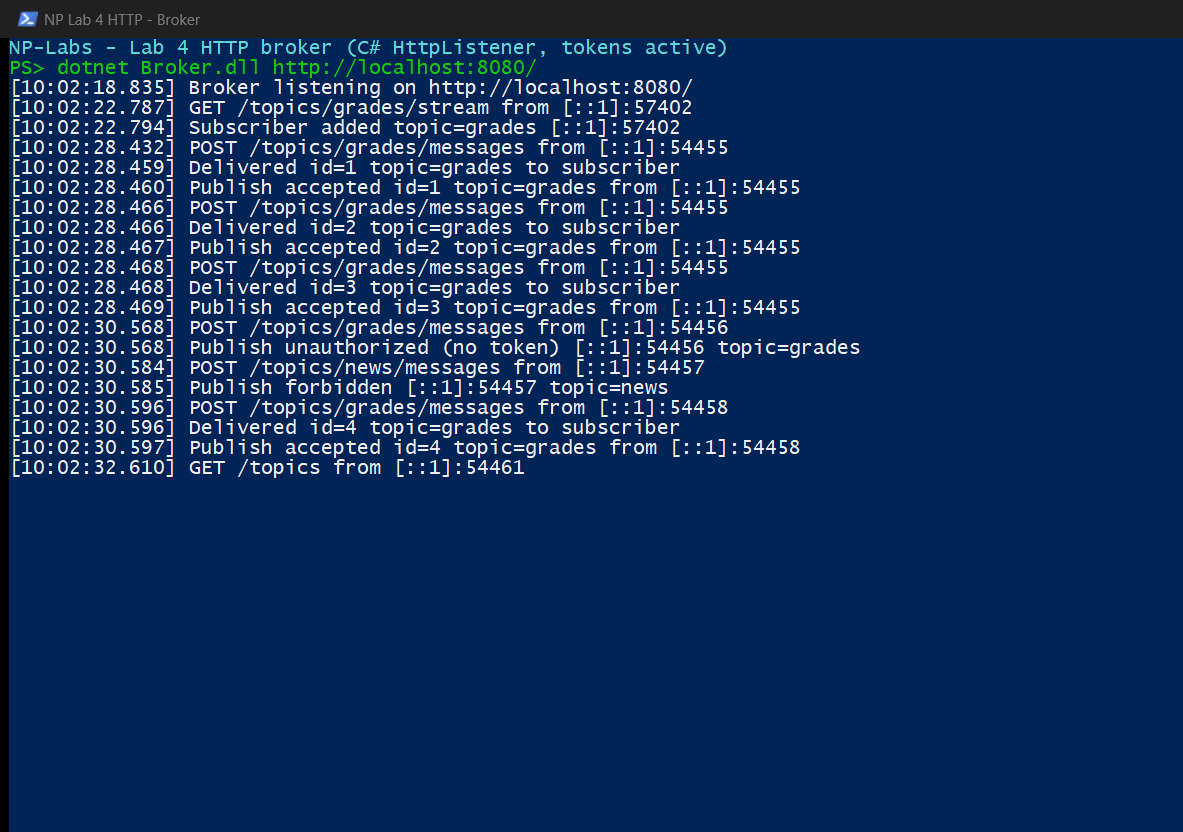
\includegraphics[width=\linewidth]{figures/lab4-http-broker.png}\\[2pt]
  {\small (a) The broker: requests, topics and deliveries.}
\end{minipage}\hfill
\begin{minipage}[t]{0.48\linewidth}
  \centering
  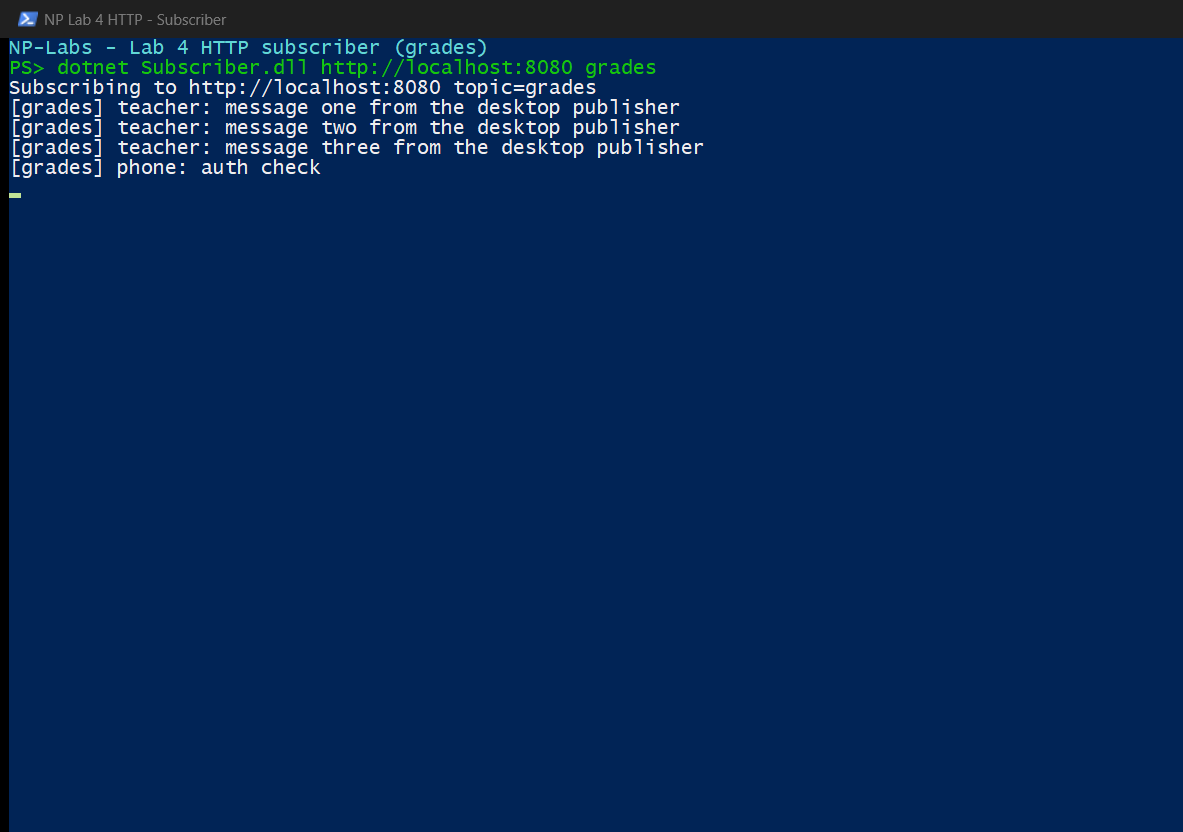
\includegraphics[width=\linewidth]{figures/lab4-http-subscriber.png}\\[2pt]
  {\small (b) A subscriber receiving the stream.}
\end{minipage}
\caption{Part 1, Task 1: the HTTP broker and a subscriber during a run.}
\label{fig:http-task1}
\end{figure}

\subsubsection{Why does a publish answer 202 and not 200?}
The message is accepted and queued. 202 means ``accepted for processing'', not
``already delivered to everyone''. A publish therefore stays fast even when one
subscriber is slow, until the delivery queue is full (1024 messages in the Go
brokers).

\subsubsection{Why one queue and one delivery loop?}
Ordering is simple to keep when one loop takes messages in the order they were
queued. Both implementations use one queue for all topics. Each subscriber is
written to in turn, so the cost of delivery grows with the number of subscribers,
not with the number of publishers.

\subsection{Task 2: Restarts}
The broker was stopped and started again in the same working directory. The next
publish got \textbf{id 12}, and \texttt{broker-data/grades/messages.json} still
held all twelve messages, so nothing was lost and the identifiers continued.

\subsubsection{Why is the temporary file renamed rather than written in place?}
Writing in place can leave a half-written file if the broker is killed midway.
With a temporary file and a rename, the file on disk is always either the old
complete version or the new complete version. On Linux the rename is atomic. On
Windows, replacing a file is close to atomic, which is enough for this laboratory
but would need more care in a production system.

\subsubsection{Does a restarted broker replay history to new subscribers?}
No. The persistence exists to keep messages and identifiers across a restart.
Subscribers receive only messages that arrive after they subscribe, as the
laboratory requires.

\subsection{Task 3: Strangers}
A publish without a token, or with an unknown one, returns 401 and a
\texttt{WWW-Authenticate: Bearer} header. A token used on a topic it does not
allow returns 403. A valid token on an allowed topic returns 202:

\par\medskip\noindent\textit{HTTP authentication: 401 with \texttt{WWW-Authenticate}, then 403, then 202.}\par\nopagebreak
\begin{terminalwindow}[]
### no token -> expect 401
HTTP/1.1 401 Unauthorized
Www-Authenticate: Bearer

### tok-phone to news -> expect 403
HTTP/1.1 403 Forbidden

### tok-phone to grades -> expect 202
HTTP/1.1 202 Accepted
{"id":11,...,"sender":"phone","body":"auth ok",...}
\end{terminalwindow}

\subsubsection{Why 401 for a missing token and 403 for a forbidden topic?}
401 means the broker does not know who is calling, so it asks for credentials.
403 means it knows the caller and refuses the action. The two codes tell a client
whether to send a token at all or to use a different one.

\subsubsection{Can a client name itself in the message?}
No. The sender is the publisher named in \texttt{tokens.txt} for the token that
was used. A client-supplied sender field is ignored when authentication is on.

\subsubsection{Is the token scheme secure?}
Not by itself. Tokens are static, stored in plain text and sent without TLS. The
scheme is adequate for a trusted laboratory network and is not a deployment
design.

% ======================================================================
\section{Part 2: The gRPC Broker}
% ======================================================================
Part 2 keeps the architecture and the three tasks, but replaces the HTTP API with
one contract. The shared file \texttt{part2-grpc/proto/broker.proto} defines all
messages and calls. The C\# and Go code is generated from it, so the publishers
and subscribers cannot disagree about field names or types.

\begin{lstlisting}[caption={The shared Protocol Buffers contract, \texttt{broker.proto}.}]
syntax = "proto3";
package broker;
option go_package = "nplabs/lab4grpc/pb;broker";
import "google/protobuf/timestamp.proto";

service Broker {
  rpc Publish (PublishRequest) returns (PublishReply);
  rpc Subscribe (SubscribeRequest) returns (stream Message);
  rpc ListTopics (ListTopicsRequest) returns (ListTopicsReply);
}

message PublishRequest {
  string topic = 1;
  string sender = 2;
  string body = 3;
  string token = 4;
}

message PublishReply {
  int64 id = 1;
  string topic = 2;
  string sender = 3;
  string body = 4;
  google.protobuf.Timestamp time = 5;
}

message SubscribeRequest {
  string topic = 1;
}

message Message {
  int64 id = 1;
  string topic = 2;
  string sender = 3;
  string body = 4;
  google.protobuf.Timestamp time = 5;
}

message ListTopicsRequest {}

message ListTopicsReply {
  repeated TopicInfo topics = 1;
}

message TopicInfo {
  string name = 1;
  int32 size = 2;
}
\end{lstlisting}

\textbf{Publish} and \textbf{ListTopics} are unary calls. \textbf{Subscribe} is
server-streaming: one HTTP/2 stream stays open, and the broker writes each new
message of the topic into it. \texttt{PublishRequest.token} is an optional
fallback for clients that cannot send metadata. When it is non-empty it is used;
otherwise the \texttt{authorization} metadata is read. The evaluation used the
metadata form.

\subsection{Task 1: Publish and deliver}
The same publishers, subscribers and topic as in Part 1 were used. Both
subscribers received all ten messages in order:

\par\medskip\noindent\textit{The Linux Go gRPC subscriber received both publishers' messages.}\par\nopagebreak
\begin{terminalwindow}[]
Subscribing to 192.168.1.41:5000 topic=grades
[grades] teacher: desktop grpc message 1
[grades] teacher: desktop grpc message 2
[grades] teacher: desktop grpc message 3
[grades] teacher: desktop grpc message 4
[grades] teacher: desktop grpc message 5
[grades] phone: linux grpc message 1
[grades] phone: linux grpc message 2
[grades] phone: linux grpc message 3
[grades] phone: linux grpc message 4
[grades] phone: linux grpc message 5
\end{terminalwindow}

\begin{figure}[H]
\centering
\begin{minipage}[t]{0.48\linewidth}
  \centering
  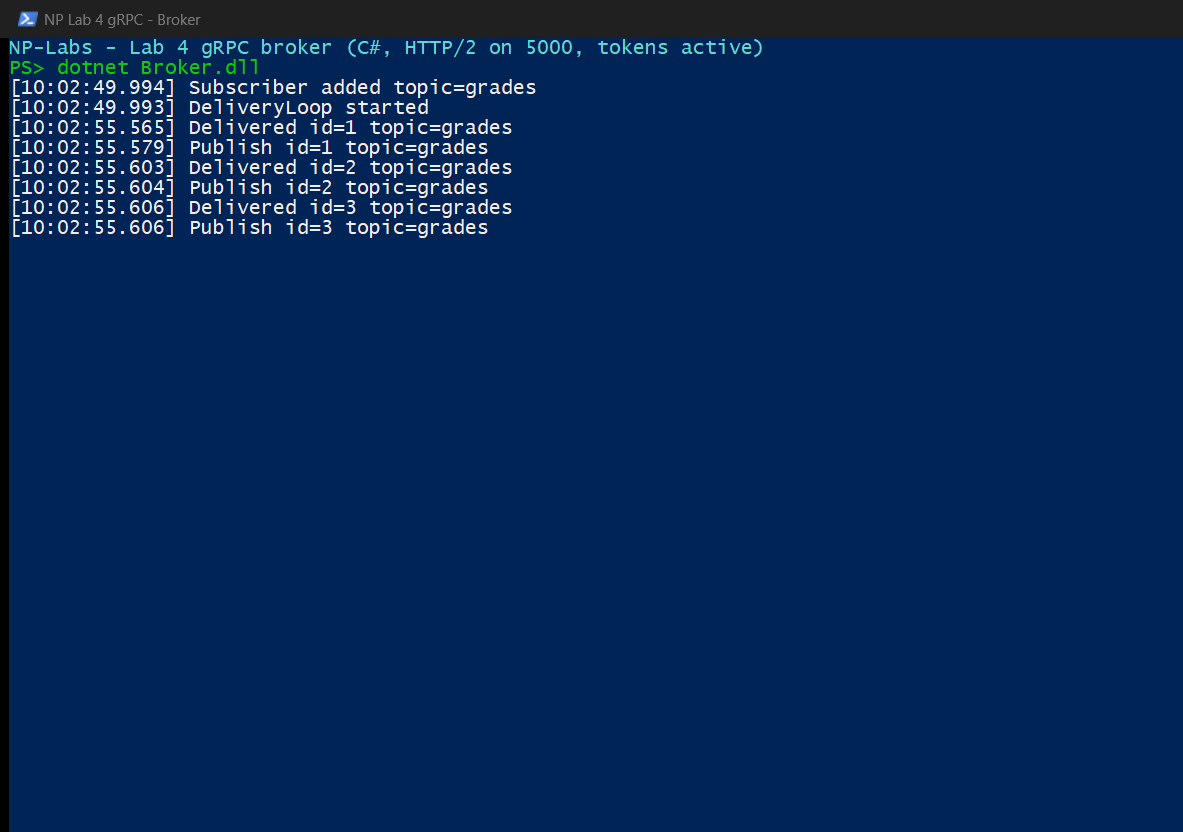
\includegraphics[width=\linewidth]{figures/lab4-grpc-broker.png}\\[2pt]
  {\small (a) The gRPC broker: unary publishes and stream subscribers.}
\end{minipage}\hfill
\begin{minipage}[t]{0.48\linewidth}
  \centering
  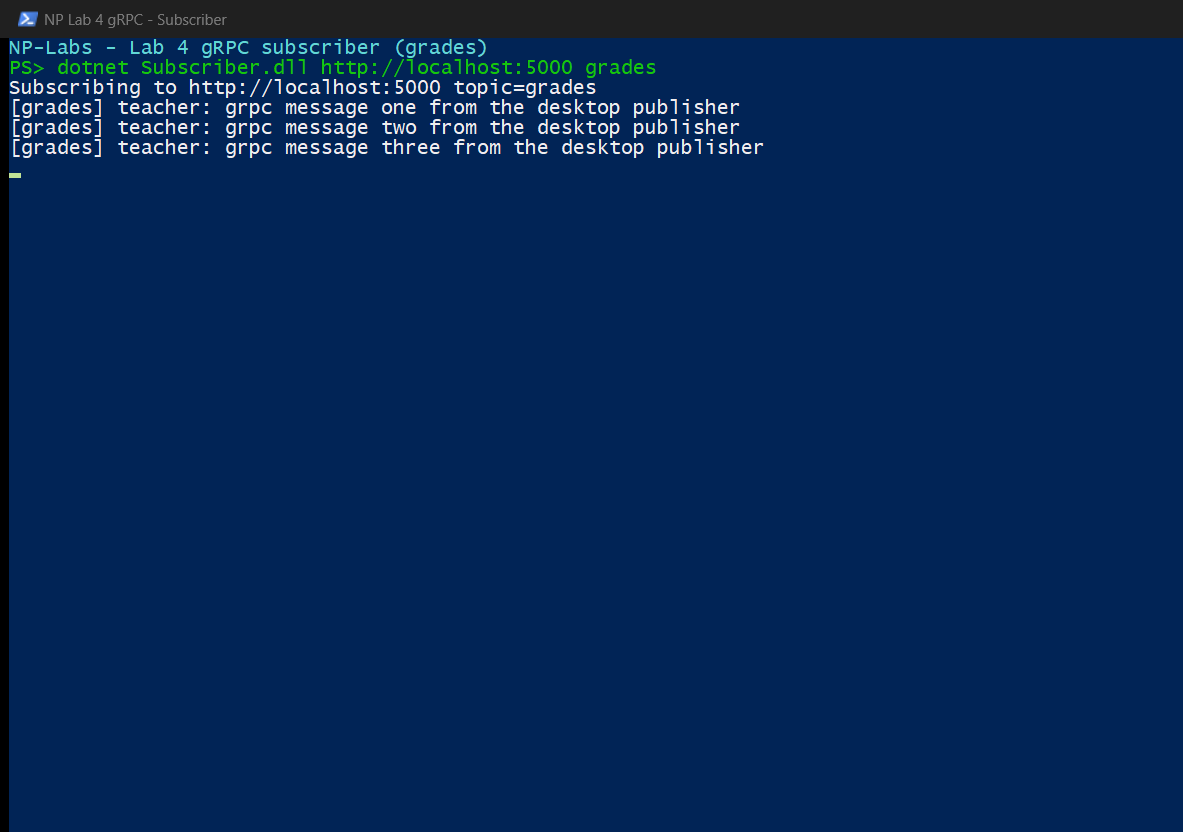
\includegraphics[width=\linewidth]{figures/lab4-grpc-subscriber.png}\\[2pt]
  {\small (b) A gRPC subscriber receiving the server stream.}
\end{minipage}
\caption{Part 2, Task 1: the gRPC broker and a subscriber during a run.}
\label{fig:grpc-task1}
\end{figure}

\subsubsection{Why is Subscribe a server stream and not repeated polling?}
The subscriber makes one call and the broker keeps the stream open. Each message
arrives as soon as it is delivered, with no polling interval and no repeated
requests. This is the gRPC form of the open HTTP response in Part 1.

\subsubsection{How does the broker notice a subscriber that has left?}
When the client cancels or disconnects, the request context ends, the
\texttt{Subscribe} handler returns, and the subscriber is removed. A failed write
has the same effect, so the other subscribers keep receiving messages.

\subsubsection{Why a bounded queue, and what does the C\# version do?}
The Go gRPC broker holds up to 1024 published messages. A publish waits only when
that queue is full, so a stalled delivery loop slows the publishers instead of
letting memory grow without limit. The C\# gRPC broker still uses an unbounded
channel, so a stalled delivery loop there would grow memory instead. The
laboratory workload is far below either limit.

\subsection{Task 2: Restarts}
The gRPC broker uses the same \texttt{broker-data} layout and the same
temporary-file-and-rename write. After a restart the next publish got
\textbf{id 12} and the persisted file still held all twelve messages.

\subsubsection{Why does the gRPC broker need the same persistence as Part 1?}
The laboratory defines one behaviour for both parts. Sharing the scheme means the
restart results are directly comparable, and only the transport changes.

\subsection{Task 3: Strangers}
The token is sent in the \texttt{authorization} metadata. A call with no token
returns \texttt{Unauthenticated}; a token for a topic it does not allow returns
\texttt{PermissionDenied}; a valid token on an allowed topic succeeds:

\par\medskip\noindent\textit{gRPC authentication: Unauthenticated, PermissionDenied, then OK.}\par\nopagebreak
\begin{terminalwindow}[]
### no token -> expect Unauthenticated
RPC error: rpc error: code = Unauthenticated desc = missing token

### tok-phone to news -> expect PermissionDenied
RPC error: rpc error: code = PermissionDenied desc = topic not allowed

### tok-phone to grades -> expect OK
Published id=11
\end{terminalwindow}

\subsubsection{Why does the metadata form need no extra field?}
Metadata is part of the transport, so the token travels outside the message and
the contract's fields stay the same as the data. The \texttt{token} field exists
only as a fallback, as described above.

\subsubsection{Which status is returned for a bad token?}
A missing or unknown token gives \texttt{Unauthenticated}. A valid token for a
forbidden topic gives \texttt{PermissionDenied}. These match the HTTP 401 and 403
cases.

% ======================================================================
\section{Evaluation}
% ======================================================================
\subsection{Research questions and procedure}
The evaluation is a controlled case study with two parts and one workload. It
asks four questions:

  \subsubsection{RQ1.} With two concurrent publishers, does every message reach every
  subscriber once, in identifier order, with unique identifiers?
  \subsubsection{RQ2.} Does a restart keep the messages and continue the identifiers?
  \subsubsection{RQ3.} Do the token rules return the required errors, and is the stored
  sender the token owner?
  \subsubsection{RQ4.} How do the HTTP and gRPC contracts compare on the same workload?

The procedure was: build both parts from a clean checkout; start the broker and
two subscribers, one C\# and one Go, on the same topic; publish five messages
from the C\# publisher and five from the Go publisher, each with its own token;
record the broker log, both subscriber transcripts, both publisher transcripts
and the persisted file; test the unauthenticated, forbidden-topic and
allowed-topic cases; then restart the broker, publish once more and check the
identifier and the stored history. The study checks correctness, not throughput.

\subsection{Environment}
Table~\ref{tab:env} lists the machines. The two desktops are the authors' own
computers on the same Wi-Fi subnet. The HTTP and gRPC brokers ran on the
Windows desktop, and the subscribers and publishers on both machines.

\begin{table}[H]
\centering
\small
\begin{tabularx}{\textwidth}{@{}l X@{}}
\toprule
\textbf{Role} & \textbf{Machine} \\
\midrule
Desktop A (Windows; C\# clients; brokers) & Dinu Plesu: HP OMEN 16-wd0xxx, Windows 11 IoT Enterprise LTSC 10.0.26300; Intel Core i5-13420H, 8 cores / 12 threads, 2.1\,GHz; 16\,GB DDR5-5600; Samsung 990 PRO 2\,TB NVMe; Wi-Fi 6E, 192.168.1.41 \\
Desktop B (Linux; Go clients) & Igor Boltunov: CachyOS, kernel 7.3.6-1-cachyos, x86-64; Intel Core i5-10300H, 4 cores / 8 threads; 7.6\,GiB RAM; Micron 2210 512\,GB NVMe; Wi-Fi 6, 192.168.1.22 \\
HTTP broker & Go, port 8080, on desktop A \\
gRPC broker & C\#, port 5000, on desktop A \\
Runtimes &.NET 10.0.404; Go 1.27.4; Rust 1.99.1 \\
\bottomrule
\end{tabularx}
\caption{Test environment for the two-desktop run.}
\label{tab:env}
\end{table}

\subsection{Results}
Table~\ref{tab:results} collects the results of both parts. Every value comes from
the transcripts and logs listed in Section~\ref{app:evidence}.

\begin{table}[H]
\centering
\small
\begin{tabularx}{\textwidth}{@{}l X X@{}}
\toprule
\textbf{Check} & \textbf{Part 1: HTTP} & \textbf{Part 2: gRPC} \\
\midrule
Messages per topic & 5 from each publisher & 5 from each publisher \\
Ids delivered & 1--10, unique, in order & 1--10, unique, in order \\
Subscribers receiving all messages & 2 of 2 & 2 of 2 \\
No token & 401, \texttt{WWW-Authenticate} & \texttt{Unauthenticated} \\
Forbidden topic & 403 & \texttt{PermissionDenied} \\
Allowed topic & 202, id 11, sender \texttt{phone} & OK, id 11 \\
After restart & next id 12; 12 messages on disk & next id 12; 12 messages on disk \\
\bottomrule
\end{tabularx}
\caption{Results of the two-desktop run for RQ1--RQ3.}
\label{tab:results}
\end{table}

\subsection{Comparison of the two contracts (RQ4)}
Both parts produced the same message ids, the same delivery order and the same
authentication outcomes. They differ in how the contract is written down and how
the messages travel.

\begin{table}[H]
\centering
\small
\begin{tabularx}{\textwidth}{@{}l X X@{}}
\toprule
\textbf{Aspect} & \textbf{HTTP (Part 1)} & \textbf{gRPC (Part 2)} \\
\midrule
Contract & paths, methods, status codes and JSON fields, agreed by hand & \texttt{broker.proto}, generated stubs \\
Transport and encoding & HTTP/1.1, JSON text & HTTP/2, binary Protocol Buffers \\
Publish & \texttt{POST}, 202 Accepted & unary \texttt{Publish} \\
Subscribe & \texttt{GET}, open response, NDJSON & server-streaming \texttt{Subscribe} \\
Auth errors & 401 / 403 & \texttt{Unauthenticated} / \texttt{PermissionDenied} \\
Topic list & \texttt{GET /topics} & unary \texttt{ListTopics} \\
Persistence & temporary file and rename & the same \\
Easy to inspect by hand & yes: \texttt{curl}, browser, logs & needs a gRPC client \\
\bottomrule
\end{tabularx}
\caption{The two parts implement the same broker with different contracts.}
\label{tab:comparison}
\end{table}

The HTTP contract is easy to test with ordinary tools and makes the streaming
visible in the protocol. The gRPC contract is stricter: a change to a field
breaks the generated code at compile time rather than at run time, and streaming
is a first-class call. For this small broker both are adequate. The choice in a
real system would depend on the tools and clients around it.

\subsection{Changes after the two-device run}\label{sec:changes}
After the two-device run the code was reviewed against the laboratory sheet. Four
faults were found and fixed in both Go brokers. The C\# brokers were changed in the
same way, but they could not be compiled or run on the machine used for these
checks, so their changes have only been checked by reading them.

\begin{itemize}
  \item \textbf{Lost or reordered messages under concurrency.} The Go brokers wrote
  the file outside the topic lock, so a stale write could replace a newer one, and
  two writers could delete the file. They also queued deliveries outside the lock,
  so subscribers could receive messages out of identifier order. A publish now holds
  a per-topic lock for its whole length.
  \item \textbf{Silent write failures.} A failed write was logged and the publish was
  still acknowledged. Now the message is removed again and the publish fails with
  500 (HTTP) or \texttt{Internal} (gRPC).
  \item \textbf{Missing tokens file.} Without a tokens file the broker accepted
  publishes with no token. Now a token is always required, so every publish is
  refused with 401 or \texttt{Unauthenticated}.
  \item \textbf{Subscribers.} The HTTP stream sent no status until the first message,
  so a subscriber could not tell it was subscribed. The stream now sends its status
  and headers when the subscription starts, and the gRPC stream sends its response
  headers at the same point. Delivery lines now name the subscriber.
\end{itemize}

Before the fixes, on one Linux machine, 2 of 12 HTTP bursts of 200 concurrent
publishes left no \path{messages.json} and a third left it one message short. Two
of six gRPC bursts left no file. Out-of-order deliveries occurred: 34 adjacent pairs out of
204 deliveries (HTTP) and 490 out of 1{,}203 (gRPC). With no tokens file a publish was
accepted with status 202.

After the fixes, on the same machine, the Go HTTP broker passed all 18 checks of its
test suite, including authentication, the stream, 40 concurrent publishers, restart
and the no-tokens case, and all 7 further checks: a failed write gave 500 with no gap
in the identifiers, and a topic name with path characters was refused. In 12 bursts of
200 concurrent publishes, every file was complete. The Go gRPC broker passed its suite
with six bursts of 200 concurrent publishes, every file complete, no out-of-order
deliveries, every message received by the subscriber, and the response headers sent
before the first message. A restart kept all 1{,}204 messages and continued the
identifiers, a failed write gave \texttt{Internal} with no gap, and a broker without
a tokens file refused every publish.

These are single-machine results. They have not been measured across two devices.

% ======================================================================
\section{Conclusion and Future Work}
% ======================================================================
Both parts implement the full laboratory: publish and deliver, restarts, and
token-based authentication. In the two-desktop run, two publishers on two
computers reached two subscribers, and every subscriber received every message in
order. Identifiers stayed unique and consecutive, a restart continued at
identifier 12 with all earlier messages on disk, and the token rules gave the
required errors on both contracts. The gRPC part shows how a typed contract and a
server-streaming call replace a hand-written REST API and an open HTTP response.

Future work would add replication or partitioning to remove the single-node
failure point; durable subscriptions and replay for late subscribers; bounded
queues with backpressure in the C\# brokers; TLS and token rotation; and a load study with many
publishers, subscribers and brokers. A formal model of the delivery and
persistence rules would allow the identifier and restart invariants to be checked
mechanically.

The fixes made after the two-desktop run are described in Section~\ref{sec:changes}.
They have been checked on one machine only. The two-device results above come from
the code before the fixes and have not been measured again across devices.

% ======================================================================
% ======================================================================
% ======================================================================
\section{Evidence files}
\label{app:evidence}
The transcripts, logs and persisted files of the two-desktop run are in
\path{Lab4/evidence/two-desktop-2026-11-26/}. Part 1 files are under
\texttt{part1-http/} and Part 2 files under \texttt{part2-grpc/}. The cross-device
run, with a phone as the second machine, is in \path{Lab4/evidence/cross-device-2026-11-26/}.

\section{Source Code and Build Instructions}\label{sec:source}

The complete source code is in the NP-Labs repository, in the 4 folder:
\begin{center}
\large
\url{https://github.com/Prince-of-Nothing/NP-Labs}
\end{center}

\begin{lstlisting}[caption={Build and start the HTTP broker and clients.}]
cd Lab4/part1-http/go
go build -o broker ./broker
go build -o publisher ./publisher
go build -o subscriber ./subscriber
./broker -addr :8080

dotnet run --project Lab4/part1-http/subscriber -- http://192.168.1.41:8080 grades
dotnet run --project Lab4/part1-http/publisher -- http://192.168.1.41:8080 grades teacher tok-teacher
\end{lstlisting}

\begin{lstlisting}[caption={Build and start the gRPC broker and clients.}]
cd Lab4/part2-grpc
dotnet run --project broker            # gRPC broker on port 5000
dotnet run --project subscriber -- 192.168.1.41:5000 grades
dotnet run --project publisher -- 192.168.1.41:5000 grades teacher tok-teacher
\end{lstlisting}

\end{document}
